% !Mode:: "TeX:UTF-8" 
\chapter{绪论}[Example]

\section{课题背景及研究目的和意义}[Number]
生物通路是细胞中分子间的一系列活动,导致细胞内某种产物或变化。生物通路可以导致新的分子的组装(如脂肪和蛋白质)、控制基因的表达、刺激细胞的移动等\footnote{http://www.genome.gov/27530687}。复杂疾病往往和生物通路网络之间存在密切的关系。复杂疾病诸如糖尿病、癌症、心脏病,高血压等与多种致病基因、蛋白、生物通路网络是相互关联的\cite{jin2011systematic}。因此深入研究生物通路网络对于探索疾病的发病机制具有重要的意义和研究价值。随着高通量技术的发展和大量生物实验的开展,基因、蛋白、代谢等组学数据日益积累,研究人员推出了一批高质量的生物通路数据库如KEGG\cite{kanehisa2008kegg}(一种受到广泛欢迎的被生物学家广泛使用的数据库)、Reactome\cite{croft2013reactome}(一个免费的和手工标注生物通路的在线数据库);DrugBank\cite{wishart2006drugbank}(一种综合性的包含大量的药物和靶点数据以及生物通路数据的数据库)等(见表\ref{table2} )。这些数据库蕴含着大量通路、疾病、药物等信息,诸如疾病致病基因,分子间的作用信息,通路网络的拓扑结构等,对于这些数据的深入研究和挖掘对揭示复杂疾病发病机理,发现药物靶点等方面具有重要的意义。

\begin{table}[htbp]
  \centering
	\caption[table1]{常用的通路数据库及网址}
\vspace{0.5em}\wuhao
\begin{tabularx}{1.0\textwidth}{lXXl}
\toprule[1.5pt]
数据库名 & 简介 & 网址 & 参考文献\\
\midrule[1pt]
KEGG & 被生物学家广泛使用的通路数据库 & http://www.kegg.jp & \cite{kanehisa2008kegg} \\
Reactome	& 免费的和手工标注生物通路的在线数据库	& https://reactome.org & \cite{croft2013reactome} \\
WikiPathways	& 使用了维基百科概念的通路数据	& https://www.wikipathways.org & \cite{pico2008wikipathways} \\
PhosphoSitePlus	& 包含小鼠和人类的通路数据的数据库 & https://www.phosphosite.org &	\cite{hornbeck2011phosphositeplus} \\
BioCyc 	& 基因组通路数据库& https://biocyc.org/	& \cite{krummenacker2005querying} \\
PANTHER	& 基因及其产物相关的通路数据库&http://www.pantherdb.org	& \cite{mi2016panther} \\
\bottomrule[1.5pt]
\end{tabularx}
\end{table}

生物通路网络通常和多种疾病、药物、靶点等数据关联,为发现与已知的通路网络关联的药物、靶点、基因关系等,需要对已知的生物通路网络进行扩展。通路网络的常见的扩展方法是将生物通路数据映射到其他生物网络(如疾病、基因、药物网络)上,作为种子节点进行扩展(如图\ref{fig1}所示)。图\ref{fig1}中蓝色的节点是通路网络中原有的节点,红色的节点是扩展后的节点。扩展前的生物通路网络如图\ref{expansion11}所示,扩展后的生物通路网络如图\ref{expansion12}所示。各种生物网络为生物通路的扩展提供了拓扑结构信息,关联数据信息、作用强度信息等。各种生物网络的拓扑结构可以预测生物通路网络中潜在的关联,生物网络中的相互作用则可以发现的生物通路网络中未知的基因、药物、疾病等潜在的链接。将这些信息进行合理的分析和应用是进行生物通路网络扩展的基础。

 生物网络的拓扑结构信息是进行生物通路扩展的重要依据。常见的扩展方法有基于网络传播的方法和基于网络节点聚类的方法。这些方法利用了网络在结构上的全部或者部分信息去寻找生物通路节点和网络中潜在的节点之间的关联,以实现生物通路的扩展。经过扩展的生物通路包含了一些潜在的关联信息。这些潜在的信息揭示了一些复杂疾病的发病机制、某些药物的靶点等。

为了对生物通路网络进行直观的认识,便于研究人员的研究和使用。网路可视化技术常常被引入到生物网络的展示过程。生物通路网络展示可以借助于生物通路图。生物通路图是一系列化合物和反应所组成的复杂网络的一种可视化表示形式。因此,一条生物通路可表示成节点和边的集合,节点可用来表示参与化学反应的反应物和产物,例如: 蛋白质,小分子化合物,DNA,RNA 等;边可表示各种相互作用关系,例如: 反应和规则。生物通路图以直观网络图谱的方式来显示相关的生物学信息,便于生物学家认清各种生物反应的网络图谱。了解生物通路中参与反应的生物分子之间的关系,各个生物分子的功能,以及各自的反应方式,以便于生物学家对生物实验数据进行观察、记录和分析。

在生物通路图中,每个节点代表一种生物分子。图中的节点有许多相关的属性可供选择设置,例如: 形状、背景颜色、大小、边框颜色、边框层次和边框的粗细等等。在生物通路图中,用边来表示各种相互作用关系、反映类型和生物学功能等等。边可分为有向边和无向边。边也可以采用不同的形状,附加采用不同的颜色和粗细。生物通路图为研究者提供了直观的认识,作为一种重要的工具加速了生物通路的研究,方便了研究者挖掘和发现已有的通路数据中潜在的信息,在揭示疾病的发病机制,提高临床治疗效果、发现药物靶点等方面具有重要的意义。

\begin{figure}{\label{fig1}}
  \centering
  \begin{minipage}{.95\linewidth}
    \setlength{\subfigcapskip}{-1bp}
    \centering
    \begin{minipage}{\textwidth}
      \centering
      \subfigure{\label{expansion11}}\addtocounter{subfigure}{-2}
      \subfigure{\subfigure[扩展前的生物通路网络]{\includegraphics[width=0.6\textwidth]{1-a}}}
      \subfigure{\label{expansion12}}\addtocounter{subfigure}{-2}
      \subfigure{\subfigure[扩展后的生物通路网络]{\includegraphics[width=0.8\textwidth]{1-b}}}
    \end{minipage}
	\caption[fig1]{通路网络扩展实例}
  \end{minipage}
\end{figure}

\section{国内外研究现状分析}[Current research situation]
\subsection{生物通路网络分析和扩展方法的国内外研究现状}[Network analysis]
 随着生物通路数据的积累和相关数据库的日益完备,对生物通路数据分析技术和生物通路网络分析和扩展方法的需求日益增长。生物通路分析技术已经成为深入研究生物学差异基因表达和蛋白的首选,因为它不仅降低了研究成本,而且增加了对于一些现象的解释能力。通路分析技术已经被广泛的使用到对基因本体分析、生物互作网络分析(如蛋白网路)等领域。第一代的生物通路分析技术是以以ORA\cite{goeman2007analyzing}方法为代表。该方法的工作流程一般是使用一定的阈值和标准创建输入列表。然后输入一个基因的列表,使得每个列表里的基因都是生物通路的一部分,接下来对于每一个通路在输入基因列表下,进行相关的测试得到最后和输入基因最为显著相关的通路,最常见的是超几何分布、卡方检测、二项式分布检测等。然而这类的方法是具有显著的缺陷的。首先,采用不同的测试的状况下其量度不同,这就意味着除了测试基因在数量上的信息,其他的测试量之间无法进行统一的比较。其次,这种方法在考虑基因时只选择了显著的基因,而丢失其他的基因。第三,没有考虑到列表里面基因之间的关联性和通路之间的关联性。

 由于ORA技术存在的这些缺点,更为先进的通路分析技术被发展出来,其中以FCS\cite{lee2011prioritizing}为典型的代表。FCS克服了ORA缺点,并实现了在从分子测量角度寻找到生物通路上的显著基因。FCS用一个统一的分数将各种不同的统计分析方法得到的结果结合了起来。OFA 和FCS方法仅仅考虑了生物通路上基因的数量和基因表达信息来确定关键的生物通路。然而,生物通路往往和其他的基因之间存在着链接,这些基因往往和生物通路起作用。为了添加更多有用的信息,基于生物通路网络拓扑结构的方法(基于通路网络分析的方法)越来越受到重视,该方法充分利用拓扑结构信息来计算在基因层面的特性。

为了深入的研究生物通路网络,对生物通路网络结构的分析是十分重要的环节。由于生物通路网络,也是一种基于边和节点的图模型。分析传统的网络的方法,对于生物通路网络的分析过程也是十分有益的。传统的网络分析方法可以完成网络抽取、网络的中心性分析,社区探测、分类、链接预测等。这些也适应于方法在生物通路网络的分析过程中。2004年Newman\cite{newman2006modularity}等人于提出了模块度(modularity)这一概念,.这一个概念在研究者引入到复杂网络中社区发现过程中,并在成功地在社交网络分析和生物网络分析中得到了实践Tamas Nepusz\cite{nepusz2012detecting}等提出了一个基于贪心策略的子网络节点聚类算法ClusterONE。ClusterONE通过定义一个量化的度量“内聚力”,聚力是用于表征子网内部的凝集程度和子网与外部的分割程度。Wu等人利用KEGG\cite{kanehisa2008kegg}中的药物-靶点,疾病-基因关系构建了一个多重网络,使用ClusterONE和Louvain\cite{blondel2008fast}算法在这个网络进行“模块发现”,对潜在的关联关系进行了预测。Emig \cite{emig2013drug}等人提出了一种基于结合局部和全局网络信息的网络分析方法。该方法融合药物靶点、基因表达芯片数据、疾病信息构造全局网络。利用邻居得分(局部网络方法)、节点关联性(局部网络方法)、网络传播(全局网络方法)、随机游走(全局网络方法)四种方法分别对全局网络进行分析,预测了网络中潜在的链接。

基于随机游走的一类方法在通路网络扩展和通路中潜在的关联关系的预测应用方面具有重要的价值。所谓的随机游走就是在规则的点阵上进行无规律行走的模型,其在每个步骤,从一个位置跳转到另一相邻位置,位置变化形成的一个序列如图\ref{fig2} XXXX所示,一维的随机游走可以看成马尔科夫链,其状态空间和整数T有关系,并且状态的转移概率(有状态T 转移到状态J 的概率)由 给出

基于随机游走的概念,一系列的方法被研究者提出并应用在生物网络扩展和生物网络中潜在链接的预测领域例如药物的重定位领域, 本人在[]中系统的总结了基于网络的方法在药物重定位的应用,[]中的很多方法,也可以被生物通路网络扩展的方面进行应用。

\begin{figure}{\label{fig2}}
  \centering
  \begin{minipage}{.7\linewidth}
    \setlength{\subfigcapskip}{-1bp}
    \centering
    \begin{minipage}{\textwidth}
      \centering
      \subfigure{{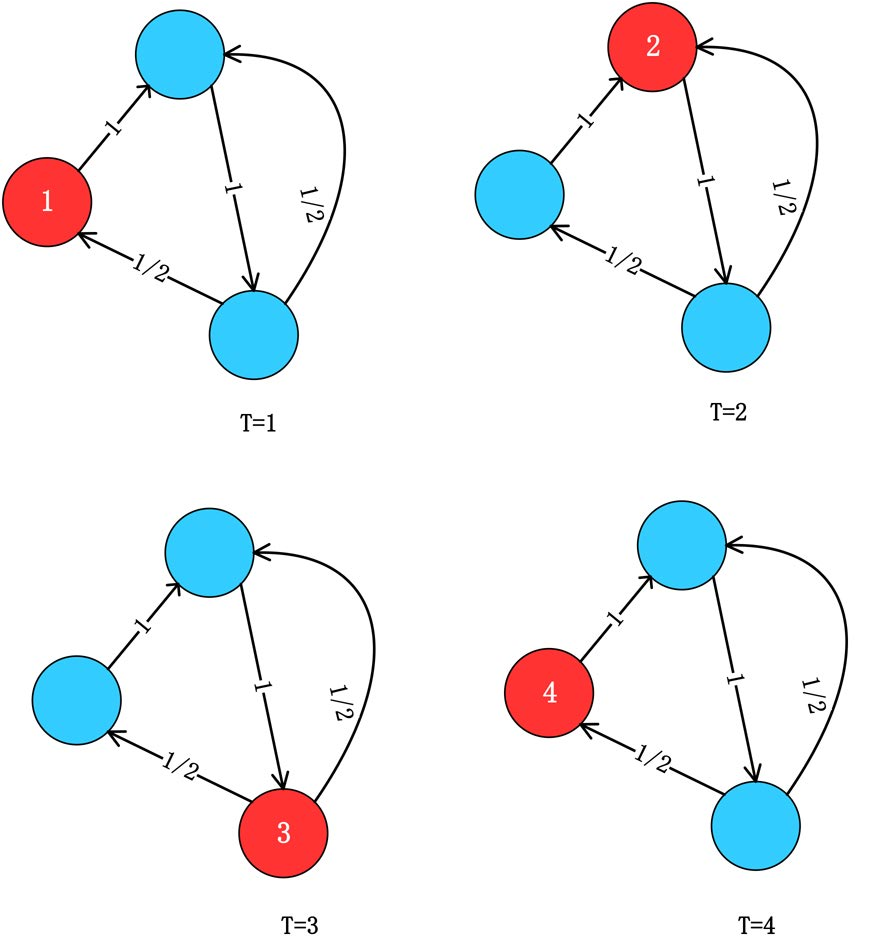
\includegraphics[width=0.7\textwidth]{rw}}}
    \end{minipage}
	\caption[fig2]{随机游走的实例}
  \end{minipage}
\end{figure}

